\begin{frame}
\frametitle{ RMI $\rightarrow$ Messages }
	\begin{center}
        % so how do we achieve RMI. method invocations are transmitted to remote locations as messages
        \includegraphics<1>[width=0.9\textwidth]{../figures/progmodel/14-rmi-collective.pdf}
        % but they're completely asynchronous. no ack / assent required from receiving processor
        % hence, a processor could receive multiple remote methods simultaneously for execution
        % so how do we handle this
	\end{center}
\end{frame}


\begin{frame}
\frametitle{Remember the void return types?}
    \begin{itemize}
        \item \alert{void return types imply one-way information transfer}
        \item signal application's intent to perform (possibly) remote task
        \item carry required input data for remote task
        \item \alert{express parallel dependencies}
        \pause
        \begin{block}{}
            Entry methods express when something \alert{can} execute.\\
            Not when something \alert{should} execute.
        \end{block}
    \end{itemize}
\end{frame}


\begin{frame}
\frametitle{
    \only<1>{ Message queues }
    \only<2>{ Scheduler }
}
	\begin{center}
        % the natural way to handle this is to use a msg q
        % so this introduces the first component at the runtime layer. above line is app. below line is rts
        % charm maintains a msg queue under the hood to handle all the msgs that comprise parallel execution
        \includegraphics<1>[width=0.9\textwidth]{../figures/progmodel/15-msg-queues.pdf}
        % how is parallel execution actually orchestrated?
        % remember that all methods are completely one-way info flows. once an RMI is packaged into a msg,
        % it has everything thats needed from the sender. this means, it can basically be invoked anytime.
        % so msgs can be picked out of this queue, the receiving object identified
        % and the method invocation can be executed
        % This is performed by the runtime scheduler. which is the engine that drives the whole parallel execution
        \includegraphics<2>[width=0.9\textwidth]{../figures/progmodel/16-scheduler.pdf}
	\end{center}
\end{frame}


\begin{frame}
\frametitle{\charm}
\begin{itemize}
    \item objects = fundamental unit of state / functionality
    \item methods = fundamental unit of execution
\end{itemize}
\pause
\begin{block}{Entry Methods ...}
\begin{itemize}[<+->]
    \item are \emph{scheduled} for execution
    \item are not preempted
    \item are not reentrant
    \item have unspecified delivery order
    \item do not require threading / locking mechanisms (typically)
\end{itemize}
\end{block}
\end{frame}


\begin{frame}
\frametitle{Prioritized Execution}
	\begin{center}
        \includegraphics<1>[width=0.9\textwidth]{../figures/progmodel/16-scheduler.pdf}
        \includegraphics<2>[width=0.9\textwidth]{../figures/progmodel/17-prio-scheduling.pdf}
	\end{center}
\end{frame}



\begin{frame}
\frametitle{Cosmology: ChaNGa}
\begin{center}
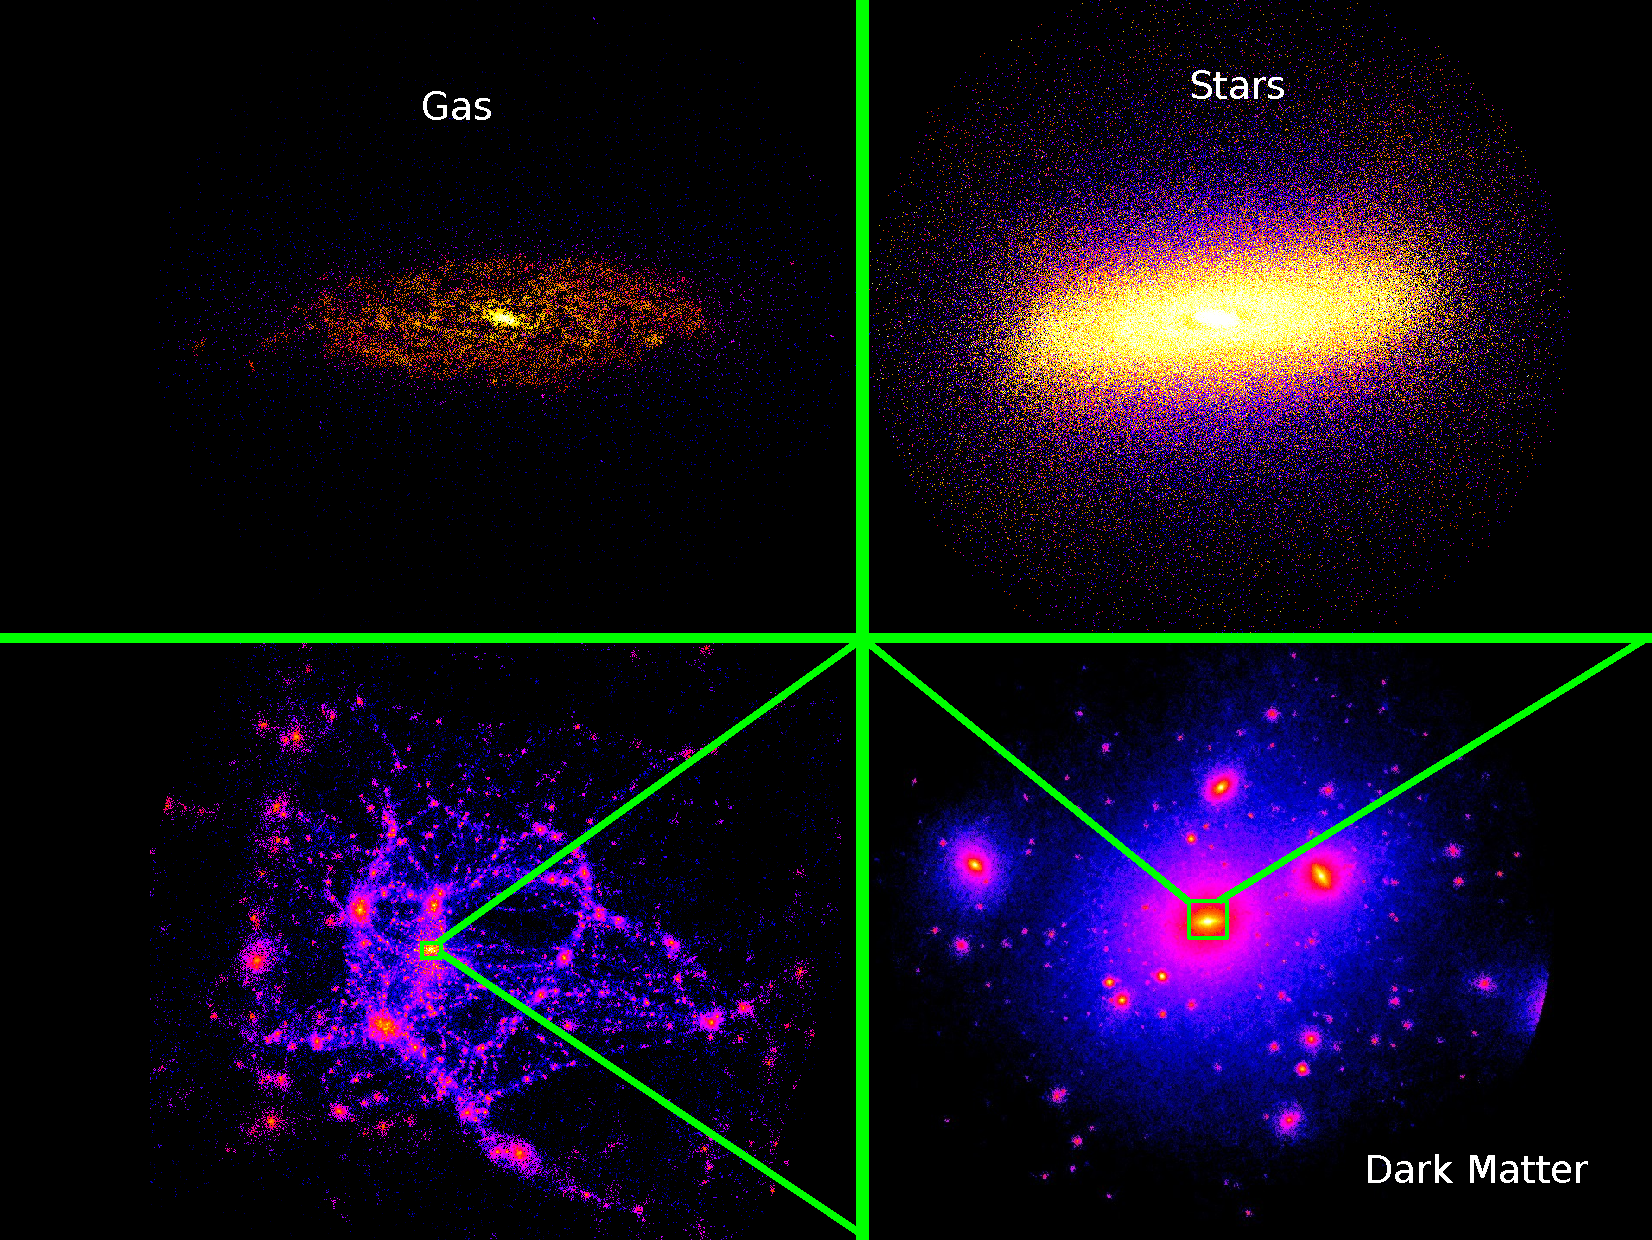
\includegraphics[width=0.9\textwidth]{../figures/changa-length-scales.pdf}
\end{center}
\end{frame}


\begin{frame}
\frametitle{Cosmology: ChaNGa}
\begin{center}
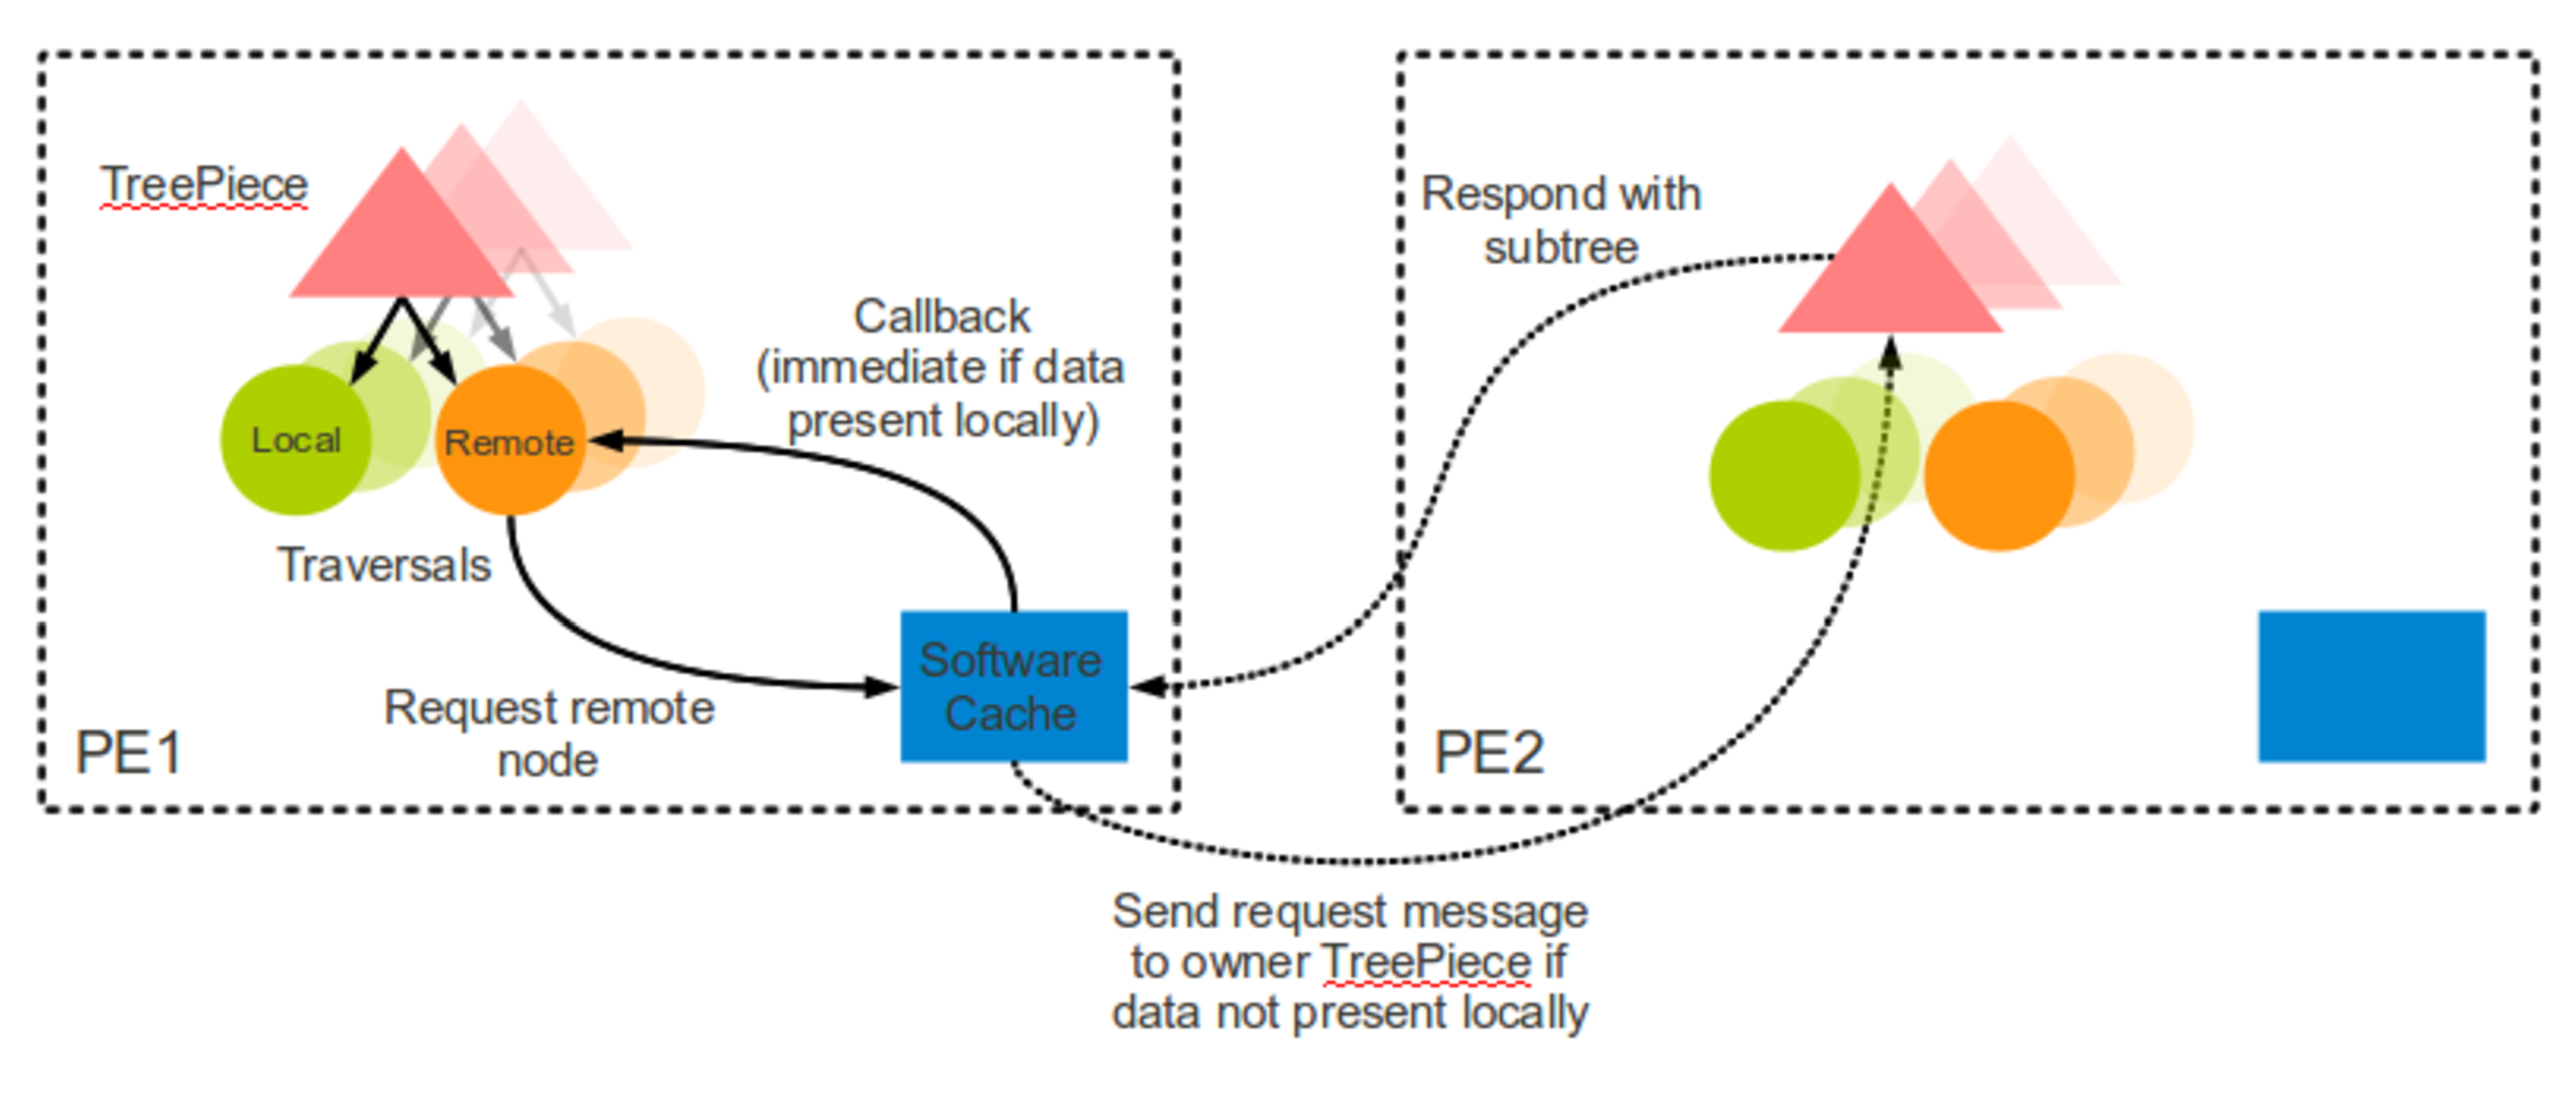
\includegraphics[width=0.9\textwidth]{../figures/changa.pdf}
\end{center}
\end{frame}


\begin{frame}
\frametitle{Cosmology: ChaNGa}
\begin{center}
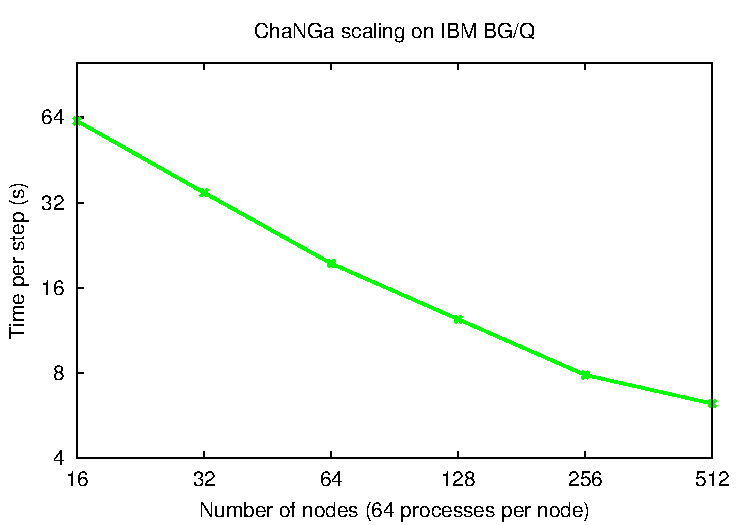
\includegraphics[width=0.9\textwidth]{../figures/changa-scaling.pdf}
\end{center}
\end{frame}


